\chapter{Stationäres Strömungsfeld}\label{statstr}
 In der Elektrostatik betrachtet man \textbf{ruhende Ladungen}. Die Grundgleichungen dafür sind mit \ref{GGes1} und \ref{GGes2} gegeben. Nun sind auch \textbf{bewegte Ladungen zugelassen}, es existiert also eine Stromdichte $\vec{J}\neq 0$. Allerdings wird sich auf den \textbf{stationären} Fall beschränkt. Das heißt:
 \begin{itemize}
 	\item Ladungen bewegen sich zwar, allerdings kommt es nicht zu einem \enquote{Ladungsstau}, die mittlere Ladung ist in jedem Leiterabschnitt zeitlich konstant ($({\partial}/{\partial t}) \rho_\text{V} = 0$, makroskopisch!). 
  \item Alle Größen, die die Strömung charakterisieren sind an jeder Stelle des Raumes zeitlich konstant ($({\partial}/{\partial t})v=({\partial}/{\partial t})J=0$).
  \end{itemize}
  Dafür muss die elektrische Feldstärke, die die Ladungen treibt, i.A. unveränderlich sein, anderenfalls würde sie durch die Kraftwirkung auf die Ladungen deren Bewegung ändern ($({\partial}/{\partial t})v= 0$ verletzt). Ein stationäres Strömungsfeld setzt also ein statisches elektrisches Feld voraus ($({\partial}/{\partial t})E=0$).\\ Nach \ref{GGstatstr1} und \ref{GGstatstr3} ist das E-Feld divergenz- und rotationsfrei. Entsprechend muss (makroskopisch) $\rho_\text{V}=0$ sein ($\nearrow$\ref{relax}), positive und negative Ladungen sind kompensiert. Ein von Gleichstrom durchflossener Leiter, der sich räumlich nicht bewegt, ist ein Anwendungsfall für das stationäre Strömungsfeld.
 \section{Grundlagen, Elektrischer Strom und Stromdichte}
 \subsection{Bewegung von Ladungsträgern}\label{bewlad}
	   Grundsätzlich sind zwei Arten der Bewegung von Ladungsträgern zu betrachten:
	        \begin{itemize}
		        \item \textbf{Thermische Bewegung} \({\vec{v}}_\mathrm{th}\): Trägt makroskopisch nicht zur Stromdichte \(\vec{J}\) bei, da \(\langle \vec{v}_\mathrm{th}\rangle = \vec{0} \) ($\langle\dots\rangle$ - Mittlung).
		        \item \textbf{Driftbewegung} \({\vec{v}}_\mathrm{D}\): Trägt zur Stromdichte \(\vec{J} \) bei, da für den Mittelwert der Driftgeschwindigkeit \(\langle \vec{v}_\mathrm{D}\rangle \ne \vec{0} \) gilt.
	        \end{itemize}
	        In Bereichen ohne Urspannung ($\nearrow$\ref{Urspannung}) gilt unter Vereinfachung von \ref{matohm} zu \ref{ohm} $\vec{J}=\kappa\vec{E}$. Die Driftbewegung muss von einer Kraft getrieben werden. Diese Kraft kommt aus dem elektrischen Feld: \(\vec{F} _\mathrm{E} =  q \cdot \vec{E} \). Die Kraft herrührend von dem magnetischen Feld (\(\vec{F} _\mathrm{H} =  q \cdot \left(\vec{v} \times \vec{B} \right) \)) ist in elektrischen Leitern in der Regel sehr klein.
	   \subsection{Stromdichte und Strom}
  \begin{center}
	  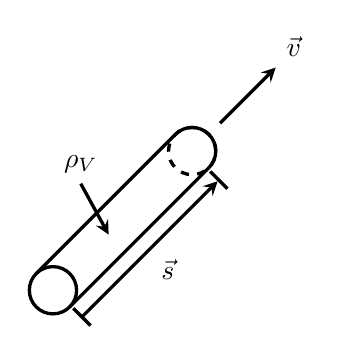
\begin{tikzpicture}[line width = 1.2pt, line join=round,x={(-0.35355cm,-0.35355cm)},y={(1cm, 0cm)},z={(0cm,1cm)},>=stealth]
	% Querschnittsflächen
	\draw [dashed] (0,0) circle (0.3cm);
	\draw (0,0,0)++(0,{0.3*sqrt(2)/2},{-0.3*sqrt(2)/2}) arc (-45:135:0.3cm);
	\draw (5,0) circle (0.3cm);
	% Begrenzungen
	\coordinate (a) at (5,0,0);
	\coordinate (ah) at (2.5,{0.5*sqrt(2)/2},{-0.5*sqrt(2)/2});
	\draw (0,{0.3*sqrt(2)/2},{-0.3*sqrt(2)/2}) -- ++(a);
	\draw (0,{-0.3*sqrt(2)/2},{0.3*sqrt(2)/2}) -- ++(a);
	% differentielles Wegstück
	\draw [|<-|] (0,{0.5*sqrt(2)/2},{-0.5*sqrt(2)/2}) -- ++(a);
	\draw (ah) node[anchor=north west] {$\dd \vec{s}$};
	% Geschwindigkeit
	\draw [->] (-1,0,0) -- (-3,0,0) node[anchor=south west] {$\vec{v}$};
	% ladungsdichte
	\draw [<-] (3,0,0) -- (4,0,1) node[anchor=south] {$\rho_\text{V}$};
\end{tikzpicture}
	  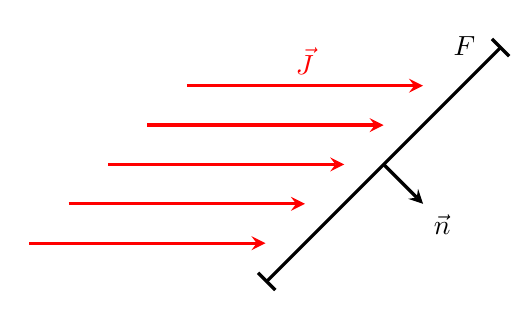
\begin{tikzpicture}[line width = 1.2pt, line join=round,x=1cm,y=1cm,>=stealth]
	% Fläche
	\draw [|-|] (0,-0.5) -- (3,2.5);
	\draw (2.8,2.5) node[anchor=east] {$ F$};
	\draw[->] (1.5,1) -- (2,0.5) node[anchor=north west] {$\vec{n}$};
	% elektrische Stromdichte
	\foreach \s in {0,0.5,1,1.5,2} \draw[->,color=red] ({-3+\s},{\s}) -- ({\s},{\s});
	\draw [color=red] (0.5,2) node[anchor=south] {$\vec{J}$};
\end{tikzpicture}
  \end{center}
  Für einen Leiter gilt ($\rho_V$ ist jetzt nicht makroskopisch gemittelt, sondern bezieht sich auf die freien Ladungsträger $\to$ \textit{Anschauung:} Bei Elektronenfluss mit statischen Atomkernen ist die Nettoladungsdichte 0, dennoch bewegen sich die Elektronen, deren Dichte mit $\rho_\text{V}$ in die Gleichung eingeht.):
  \begin{equation}\label{jrhov}
	  \vec{J} = \rho_\text{V} \cdot \vec{v}
  \end{equation}

  Der Gesamtstrom durch die Fläche \(\vec{F} \) berechnet sich nach
  \begin{equation}\begin{split}
		  I &= \iint\limits_{ F} \vec{J} \cdot \dd{}{\vec{F}}
		  = \iint\limits_{ F} \vec{J} \cdot \vec{n} \dd{}{ F}
		  = \iint\limits_{ F} J^n \dd{}{ F}
	  \end{split}\end{equation}
  mit
  \begin{equation}
	  J^\text{n} = \vec{J} \cdot \vec{n}
  \end{equation}
  \subsection{Kontinuitätsgleichung}\label{kontherl}
  \subsubsection{Herleitung Kontinuitätsgleichung über Ladungserhaltung}
	  \begin{center}
		  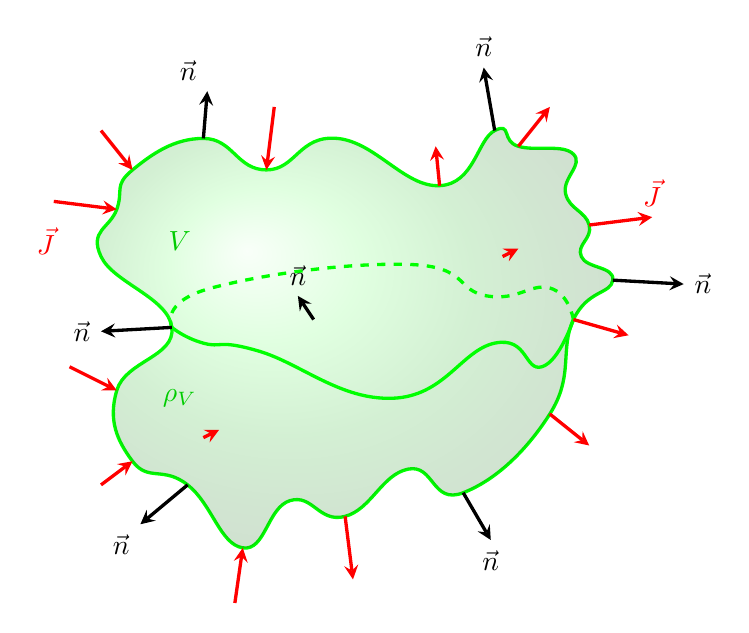
\begin{tikzpicture}[line width = 1.2pt, line join=round,x=1cm,y=1cm,>=stealth]
	% Koordinaten des Volumens
	\coordinate (a) at (3,0);
	\coordinate (b) at (3.5,0.5);
	\coordinate (c) at (3.1,0.8);
	\coordinate (d) at (3.2,1.2);
	\coordinate (e) at (2.9,1.6);
	\coordinate (f) at (3.0,2.1);
	\coordinate (g) at (2.3,2.2);
	\coordinate (h) at (2,2.4);
	\coordinate (i) at (1.3,1.7);
	\coordinate (j) at (0,2.3);
	\coordinate (k) at (-0.9,1.9);
	\coordinate (l) at (-1.7,2.3);
	\coordinate (m) at (-2.6,1.9);
	\coordinate (n) at (-2.5,1.6);
	\coordinate (o) at (-2.8,1.4);
	\coordinate (p) at (-3,0.8);
	\coordinate (q) at (-2.1,-0.1);
	\coordinate (r) at (-2.8,-0.9);
	\coordinate (s) at (-2.6,-1.8);
	\coordinate (t) at (-1.9,-2.1);
	\coordinate (u) at (-1.2,-2.9);
	\coordinate (v) at (-0.6,-2.3);
	\coordinate (w) at (0.1,-2.5);
	\coordinate (x) at (0.9,-1.9);
	\coordinate (y) at (1.6,-2.2);
	\coordinate (z) at (2.7,-1.2);
	% Volumen
	\draw [color=green] plot [smooth cycle, tension=0.8] coordinates {(a) (b) (c) (d) (e) (f) (g) (h) (i) (j) (k) (l) (m) (o) (p) (q) (r) (s) (t) (u) (v) (w) (x) (y) (z)};
	\shade [ball color=white!20!green, opacity=0.20] plot [smooth cycle, tension=0.8] coordinates {(a) (b) (c) (d) (e) (f) (g) (h) (i) (j) (k) (l) (m) (o) (p) (q) (r) (s) (t) (u) (v) (w) (x) (y) (z)};
	\draw [color=green] plot [smooth, tension=0.8] coordinates {(a) (2.6,-0.6) (2,-0.3) (0.7,-1) (-1,-0.4) (-1.7,-0.3) (q)};
	\draw [color=green, dashed] plot [smooth, tension=0.8] coordinates {(a) (2.7,0.4) (1.9,0.3) (0.9,0.7) (-1.6,0.4) (q)};
	\draw [color=green!80!black] (-2,1) node {$ V $};
	\draw [color=green!80!black] (-2,-1) node {$ \rho_\text{V} $};
	% Normalenvektoren
	\draw [->] (q) -- ++(-0.9,-0.05) node[anchor=east] {$ \vec{n} $};
	\draw [->] (h) -- ++(-0.14,0.8) node [anchor=south] {$ \vec{n} $};
	\draw [->] (b) -- ++(0.9,-0.05) node[anchor=west] {$ \vec{n} $};
	\draw [->] (y) -- ++(0.35,-0.6) node[anchor=north] {$ \vec{n} $};
	\draw [->] (t) -- ++(-0.6,-0.5) node[anchor=north east] {$ \vec{n} $};
	\draw [->] (l) -- ++(0.05,0.6) node[anchor=south east] {$ \vec{n} $};
	\draw [->] (-0.3,0) -- ++(-0.2,0.3) node[anchor=south] {$ \vec{n} $};
	% Stromdichten
	\draw [color=red] (-3.7,1) node {$ \vec{J} $};
	\draw [color=red] (4,1.6) node {$ \vec{J} $};
	% hineinflie�end
	\draw [<-,color=red] (m) -- ++(-0.4,0.5);
	\draw [<-,color=red] (s) -- ++(-0.4,-0.3);
	\draw [<-,color=red] (o) -- ++(-0.8,0.1);
	\draw [<-,color=red] (r) -- ++(-0.6,0.3);
	\draw [<-,color=red] (k) -- ++(0.1,0.8);
	\draw [<-,color=red] (u) -- ++(-0.1,-0.7);
	\draw [->,color=red] (-1.7,-1.5) -- ++(0.2,0.1);
	% herausflie�end
	\draw [->,color=red] (z) -- ++ (0.5,-0.4);
	\draw [->,color=red] (g) -- ++ (0.4,0.5);
	\draw [->,color=red] (d) -- ++ (0.8,0.1);
	\draw [->,color=red] (a) -- ++ (0.7,-0.2);
	\draw [->,color=red] (w) -- ++ (0.1,-0.8);
	\draw [->,color=red] (i) -- ++ (-0.05,0.5);
	\draw [->,color=red] (2.1,0.8) -- ++(0.2,0.1);
\end{tikzpicture}
	  \end{center}
		  In \ref{ladungserhaltung} wurde die Kontinuitätsgleichung aus der \textbf{Ladungserhaltung} hergeleitet. Die Aussage ist, dass wenn ein Nettostrom durch eine geschlossene Oberfläche eines Volumens ($V\neq 0$) geht, die Ladungsdichte dieses Volumens zeitabhängig sein muss. Es gilt also:
		        \begin{equation}
			        \dfrac{\partial \rho_\text{V}}{\partial t} \neq 0
		        \end{equation}
		   Wegen der Ladungserhaltung musste gelten:
		        \begin{equation}\begin{split}
				        \oiint\limits_{O(V)} \vec{J} \cdot \dd{}{\vec{F}} = -\iiint\limits_{V} \dfrac{\partial \rho_\text{V}}{\partial t} \dd V
				        \to \iiint\limits_{V} \div \vec{J} \dd V  = -\iiint\limits_{V} \dfrac{\partial \rho_\text{V}}{\partial t} \dd V
			        \end{split}\end{equation}
		   Das liefert die \textbf{Kontinuitätsgleichung}:
		        \begin{equation}\label{kont}
			        \boxed{\div \vec{J} = -\dfrac{\partial \rho_\text{V}}{\partial t}}
		        \end{equation}
  \subsubsection{Herleitung Kontinuitätsgleichung über Maxwell}
  Mit \ref{durchf} folgt:
		        \begin{equation}\begin{split}\rot \vec{H}=\vec{J} +\frac{\partial \vec{D}}{\partial t}	\stackrel{\div \rot = 0}{\Longrightarrow} 0 = \div \vec{J} + \div \dfrac{\partial \vec{D} }{\partial t}
			        \end{split}\end{equation}
	Anwendung von \ref{gauss} liefert die \textbf{Kontinuitätsgleichung}:
		        \begin{equation}\begin{split}
				        0 = \div \vec{J} + \dfrac{\partial \rho_\text{V}}{\partial t}
			        \end{split}\end{equation}
		          \subsubsection{Adaption für statiönäres Strömungsfeld}
		   In einem stationären Strömungsfeld gilt definitionsgemäß:
		        \begin{equation}\label{kontstat}
			        \dfrac{\partial \rho_\text{V}}{\partial t} = 0 \to \boxed{\div \vec{J} = 0}
		        \end{equation}
		   Die integrale Form entspricht dem \textbf{Kirchhoffschen Knotensatz}:
		        \begin{equation}
			        \oiint\limits_{O(V)} \vec{J} \cdot \dd{}{\vec{F}} = 0
		        \end{equation}
		        Zu beachten ist, dass mit \ref{kontstat} nach \ref{divsV} zunächst allgemein gilt:
		        \begin{equation}
		        	\div \vec{J}= \div \kappa \vec{E} = \grad \kappa \cdot\vec{E} + \kappa\div \vec{E} = 0
		        \end{equation}
		        Ist $\kappa$ ortsunabhängig entfällt der erste Term.
		         \subsubsection{Beispiel}
		        Es wird ein zylinderförmiger Leiter der Länge $l$ betrachtet, welcher von einem Gleistrom $I$ in $\vu{z}$-Richtung durchflossen wird. Der Leitermittelpunkt liegt in Zylinderkoordinaten bei $\rho=0$, der Leiter hat den Radius $\rho=a$. Außer $\kappa$ sind die Materialparameter homogen, es gibt aber eine inhomogene Leitfähigkeit:
		        \begin{equation}
		        	\kappa(\rho)=\kappa_0\left(1-\frac{\rho}{2a}\right)
		        \end{equation}
		        Es soll formal gezeigt werden, dass $\vec{{E}}$ keine $\vu{\rho}$-Komponente hat. Wegen \ref{kontstat} mit \ref{divsV} gilt zunächst:
		        \begin{equation}\label{statstrbsp1}
		        	\div \vec{J}= \div \kappa(\rho) \vec{E} = \grad \kappa(\rho) \cdot\vec{E} + \kappa(\rho)\div \vec{E} = 0
		        \end{equation}
		        Makroskopisch gilt $\rho_\text{V}=0$ ($\nearrow$\ref{relax}). Damit und mit \ref{gauss} folgt $\div\vec{D}=\varepsilon\div\vec{E}=0\Rightarrow\div\vec{E}=0$. Somit folgt aus \ref{statstrbsp1} unter Anwendung des Gradientenoperators in Zylinderkoordinaten ($\nearrow$\ref{difOpKo}):
		        \begin{equation}\begin{split}
		        	\grad \kappa( \rho) \cdot\vec{E} &= 0\\
		        	-\kappa_0\frac{1}{2a}\vu{\rho} \cdot\vec{E} &= 0
	\end{split}\end{equation}
Damit das allgemein erfüllt ist, kann $E_\rho$ nur 0 sein. Wegen $\vec{E}=-\grad\phi$ folgt außerdem, dass $E_\rho=-\frac{\partial \phi}{\partial \rho}=0$, somit hat $\phi$ keine $\rho$-Abhängigkeit.
 \section{Modell des stationären Strömungsfeldes}
 \subsection{Drude-Modell, Leitfähigkeit}
	  Die Lorentzkraft ist in \ref{lorentz} gegeben. In \ref{bewlad} wurde bereits festgehalten, dass die magnetische Kraft hier vernachlässigt werden kann, also $\vec{F}=q\vec{E}$ gilt.  Aus der Bewegungsgleichung folgt
	        \begin{equation}\label{bewegstrom}
		        m \cdot \dfrac{\partial \vec{v}}{\partial t} =  q \vec{E} \implies \vec{v}(t) = \vec{v}_0 + \dfrac{ q}{ m} \cdot \vec{E} \cdot t
	        \end{equation}
	    Für \(\vec{E} = \const \) ist \(\vec{v} \sim t\) und \(\vec{J} \sim t \). Das würde bedeuten, dass der Strom mit wachsender Zeit immer größer wird. Der experimentelle Befund ist aber
	        \begin{equation}
		        U =  R \cdot  I \text{ mit }  U \sim E \text{ und }  I \sim J
	        \end{equation}
	   Anders ausgedrückt bedeutet dies (Es ist zu beachten, dass allgemein $\vec{J}=\kappa\frac{\vec{F}}{q}$ gilt und erst durch Vernachlässigung der Komponente des B-Feldes in \ref{lorentz} die Gleichung \ref{ohm} folgt. Außerdem ist $\kappa$ i.A. ein Tensor und erst in isotropen Medien ein Skalar.): 
	        \begin{equation}\label{ohm}
	        	\boxed{\vec{J} = \kappa \cdot \vec{E}}
	        \end{equation}
Für eine verschwindende Stromdichte ($\vec{J} = \vec{0}$) gilt \(\vec{E} = \vec{0} \). Für perfekte Leiter (\(\kappa \,\rightarrow\, \infty \)) gilt \(\vec{E} = \vec{0} \) auch für  $\vec{J} \ne \vec{0}$. Für einen guten Leiter (\(\kappa < \infty \)) ist ein kleines elektrisches Feld notwendig um \(\vec{J} = \const \) zu halten. ($I=1\mathrm{A}$; $A=1\mathrm{mm^2}$; $\kappa=60\cdot 10^6\mathrm{\frac{A}{Vm}} \to E=1.7 \cdot 10^{-14}\mathrm{\frac{V}{m}}$). In \textbf{realen Leitern} existiert also bei Stromfluss ein \textbf{elektrisches Feld}.\\
	        Nach \ref{bewegstrom} müsste, wenn ein konstantes elektrisches Feld anliegt, gelten, dass die Ladungsträger beschleunigt werden. Experimentell zeigt sich aber, dass bei $\vec{E} = \text{const.}$ auch $\vec{J} = \text{const.}$, d.h. $\vec{v} = \text{const.}$ gilt. Inelastische Stöße mit Atomrümpfen hemmen die Bewegung durch den realen Leiter, es entsteht eine Gegenkraft. Das elektrische Feld kompensiert diese Hemmung, sodass die resultierende Kraft 0 ist. \textbf{Trotz} eines \textbf{elektrischen Feldes} ($\to$ Beschleunigung) erhält man also eine \textbf{konstante Geschwindigkeit}.\\
	        Ein inelastischer Stoß bedeutet anschaulich, dass das Teilchen seine komplette Geschwindigkeit verliert (\enquote{es fängt von Null an}). Die Bewegung des Teilchens sieht also folgendermaßen aus, es wird bis zum Stoß mit einer konstanten Beschleunigung beschleunigt:
	        \begin{center}
		        {\begin{tikzpicture}[line width = 1.2pt, scale = 2, line join=round,x=1cm,y=1cm,>=stealth]
	% Koordinatensystem
	\draw [->] (0,0) -- (3.6,0) node[anchor=north west] {$z$};
	\draw [->] (0,0) -- (0,1.5) node[anchor=east] {$  v $};
	% Plot
	\foreach \e in {1,2,3} {\draw ({\e-1},0) -- ({\e},{1});
			\draw [dashed] ({\e},1) -- ({\e},0);}
	\draw (3,0) -- (3.5,0.5);
	\draw (1,0) node[anchor = north] {$\tau$};
	\draw (2,0) node[anchor = north] {$2 \tau$};
	\draw (3,0) node[anchor = north] {$3 \tau$};
	\draw [dashed] (3.5,1) -- (0,1) node [anchor=east] {$ \dfrac{ q}{ m} \cdot E \cdot \tau $};
\end{tikzpicture}}
	        \end{center}
	        Aus der Gitterkonstante \(l_\mathrm{F} \approx 1 \mathrm{nm}\) und der mittleren Geschwindigkeit der Teilchen lässt sich hierbei die Stoßzeit $\tau = \dfrac{l_\mathrm{F}}{\langle { v} \rangle}$ berechnen, also die Zeit, die ein Teilchen benötigt um erneut gegen das Gitter zu stoßen (\enquote{und damit schon wieder von Null anfangen zu müssen :(}). Aus der Grafik ergibt sich der Mittelwert der Geschwindigkeit (Mittlung über lineare Funktion $\hat{=}$ Faktor $\frac{1}{2}$) zu $\langle { v} \rangle = \dfrac{1}{2} \cdot \dfrac{ q}{ m} \cdot E \cdot \tau$, woraus folgt
		        $\langle { v} \rangle =  \sqrt{\dfrac{1}{2} \cdot \dfrac{ q}{ m} \cdot E \cdot l_\mathrm{F}}$. Dies steht aber im \textbf{Widerspruch} zu \(\langle { v} \rangle \sim E \), was nach \ref{ohm} gelten müsste.  Dieser Widerspruch lässt sich durch das \textbf{Drude Modell}, wonach nicht die Driftbewegung sondern die \textbf{thermische Bewegung} maßgeblich für die Geschwindigkeit ist. Wegen \(|\vec{v}_\mathrm{th}| \gg |\vec{v}_\mathrm{D}| \) passiert ein Stoß aufgrund der thermischen Bewegung viel schneller, also ist $\tau  = \dfrac{l_\mathrm{F}}{ v_\mathrm{th}}$ viel kleiner als $\tau  = \dfrac{l_\mathrm{F}}{ \langle v \rangle }$. Die mittlere Driftgeschwindigkeit ergibt sich demnach mit:
	        \begin{equation}\begin{split}
			        |\vec{v}_\mathrm{D}| = \langle {|\vec{v}_\mathrm{D}|} \rangle = \dfrac{1}{2} \cdot \dfrac{ q}{ m} \cdot E \cdot \dfrac{l_\mathrm{F}}{|\vec{v}_\mathrm{th}|}
		        \end{split}\end{equation}
	   Damit und mit der Anzahldichte der Ladungen \(n\) gilt:
	        \begin{equation}\label{ladunggeschw}\begin{split}
			        \vec{J} &= \rho_\text{V} \cdot \vec{v}_\mathrm{D} = n \cdot  q \cdot \vec{v}_\mathrm{D}\\
			        &= \dfrac{1}{2} \cdot \dfrac{n \cdot  q^2 \cdot l_\mathrm{F}}{ m \cdot |\vec{v}_\mathrm{th}|} \cdot \vec{E} = \kappa \cdot \vec{E}\quad \text{ mit }\quad \boxed{\kappa= \dfrac{1}{2} \cdot \dfrac{n \cdot  q^2 \cdot l_\mathrm{F}}{ m \cdot |\vec{v}_\mathrm{th}|}}
		        \end{split}\end{equation}
	   Die thermische Energie steht für die thermische Bewegung (kinetische Energie) zur Verfügung (auf jeden Freiheitsgrad $f$ entfällt $\frac{1}{2} \cdot k_\mathrm{B} \cdot T$, wobei $f$ wegen des dreidimensionalen Raumes gleich 3 ist):
	        \begin{equation*}
	        	\frac{1}{2} \cdot  m \cdot  v_\mathrm{th}^2 = \frac{3}{2} \cdot k_\mathrm{B} \cdot T
	        \end{equation*}
	   Für Elektronen lässt sich damit bei Raumtemperatur $ v_\mathrm{th} = 10^5 \mathrm{\frac{m}{s}}$ berechnen, was die Annahme \(|\vec{v}_\mathrm{th}| \gg |\vec{v}_\mathrm{D}| \) rechtfertigt, weil die Driftgeschwindigkeit in der Größenordnung $\frac{\mathrm{cm}}{\mathrm{s}}$ ist. Mit der Gitterkonstante \(l_\mathrm{F} = 1 \mathrm{nm} \) kann man nun die Stoßzeit
	        $\tau = 10^{-14}\mathrm{s}$ abschätzen.
 \subsection{Elektromotorische Kraft (EMK) / Urspannung}\label{Urspannung}
 Dieser Abschnitt basiert teilweise auf \href{https://de.wikipedia.org/wiki/Elektromotorische_Kraft}{Wikipedia}.
 \subsubsection{Notwendigkeit von Quellen in Stromkreisen}
	   Im stationären Fall hat das Induktionsgesetz ($\nearrow$\ref{ind}) die einfache Form $\rot \vec{E} = \vec{0}$.  Mit \(\vec{E} = \kappa^{-1} \cdot \vec{J} \) folgt für jeden beliebigen geschlossenen Weg:
	        \begin{equation}
		        \rot \left( \dfrac{1}{\kappa} \cdot \vec{J} \right) = \vec{0} \xRightarrow{\text{\ref{stokes}}} \oint\limits_{C} \underbrace{\dfrac{1}{\kappa}}_\rho \vec{J}\cdot \dd\vec{s} = 0 \implies \vec{J} = \vec{0} 
	        \end{equation}
	        Wäre $\vec{J}\neq 0$ würde entweder $\vec{J}\uparrow\uparrow \dd\vec{s}$ oder $\vec{J}\uparrow\downarrow \dd\vec{s}$ auf dem kompletten Weg gelten, sodass das Integral zwangsläufig $\neq 0$ würde. Das bedeutet, dass in einem beliebigen geschlossenen, quellenfreien Stromkreis zunächst kein Strom fließen kann. Eine stationäre Stromdichte \(\vec{J} \ne \vec{0} \) erfordert folglich eine \textbf{Energiequelle}. Diese kann verteilt (z.B. Induktion) oder konzentriert (z.B. Batterie, Photozelle) sein.
	        \subsubsection{Feldtheoretische Einordnung elektrochemischer Zelle}
	        Nichtelektrische Vorgänge (z.B. chemische) können eine Ladungstrennung hervorrufen. Diese wird dann durch die \textbf{eingeprägte elektrische Feldstärke} \(\vec{E}_\mathrm{E} \), eine Rechengröße, modelliert. Dabei gilt:
		              \begin{equation}
			              \oint\limits_{C} \vec{E}_\mathrm{E}\cdot \dd\vec{s} = \int\limits_{-\to +} \vec{E}_\mathrm{E}\cdot \dd\vec{s}  = V \neq 0 \to \text{ \textbf{EMK, Urspannung}}
		              \end{equation}
		   Die eingeprägte elektrische Feldstärke ist nur innerhalb der Quelle $\neq 0$, der Integrationsweg $-\to +$ meint den Weg vom Minuspol zum Pluspol. Anschauung (\href{https://commons.wikimedia.org/wiki/File:ElektromotorischeKraft.svg}{Bildquelle}):
		   \begin{center}
		   	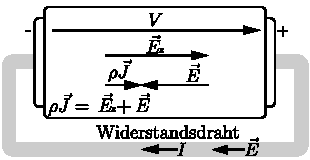
\includegraphics{res/Urspannung.pdf}
		   \end{center}
	   Im Gebiet elektromotorischer Kräfte gilt das erweiterte Ohmsche Gesetz (wobei $\rho$  der spezifische Widerstand in der Zelle ist):
	   \begin{equation}
	   	\vec{J}=\frac{\vec{E}_\mathrm{E}+\vec{E}}{\rho}
	   \end{equation}
	   Eine Ladung $q$ verschiebende Kraft ist dort entsprechend gleich $\vec{F}=q\left(\vec{E}_\mathrm{E}+\vec{E}\right)$.  Im Fall des Leerlaufes gilt $\vec{E} =- \vec{E}_\mathrm{E}$. Das bedeutet, dass die von den Polladungen hervorgerufene elektrische Feldstärke die eingeprägte elektrische Feldstärke kompensiert, sodass keinerlei Ladung in der Zelle transportiert wird. Also gilt für die Urspannung: $$V=\int\limits_{-\to +} \vec{E}_\mathrm{E}\cdot \dd\vec{s}=\int\limits_{+\to-} -\vec{E}_\mathrm{E}\cdot \dd\vec{s}=\int\limits_{+\to -} \vec{E}\cdot \dd\vec{s}=U_Q$$ \textbf{Beachte:} $V$ zeigt von \enquote{- nach +} $U_Q$ wie immer von \enquote{+ nach -}, die Urspannung treibt einen elektrischen Strom \textit{in}, die Quellenspannung \textit{entgegen} seiner Richtung an (haben $U_Q$ und $V$ die selbe Zählpfeilrichtung sind sie also vorzeichenverschieden).  Die Urspannung wird demnach im Leerlauf an den Anschlüssen als Quellspannung messbar. Wie die Quellspannung ist die Urspannung und damit auch $\vec{E}_E$ \textbf{belastungsunabhängig} (der Spannungsabfall bei Belastung erfolgt über den Innenwiderstand). Außerdem gilt für die elektrochemische Zelle wie oben (es ist der Entladefall skizziert):
\begin{equation}
	I\hat{R}=I\oint\frac{\rho(s)}{A}\mathrm{d}s=\oint\rho\vec J\mathrm{d}\vec s=\oint(\vec E_\mathrm{E} + \vec E)\mathrm{d}\vec s=\oint\vec E_\mathrm{E}\mathrm{d}\vec s=V=U_Q
\end{equation}
Mit $\hat{R}=R_i+R_a$ als Umlaufwiderstand des Stromkreises, $A$ als (ortsabhängigem) Querschnittsflächeninhalt und $\rho(s)$ als (ortsabhängigem) spezifischen Widerstand. Die Integrale sind entsprechend der Skizze im Uhrzeigersinn orientiert.\\
 Anhand der Pfeile in der Zeichnung kann man sich einige Dinge veranschaulichen, die man von der Modellierung einer Zelle als Spannungsquelle $U_Q$ mit Innenwiderstand $R_i$ und einer resistiven Last $R_a$ erwarten würde. Nachfolgend zwei Beispiele:
 \begin{itemize}
  \item Liegt Leerlauf vor fließt kein Strom, es gilt $\rho_i J = 0$, also ist $E_\mathrm{E}=-E$ in der Zelle. Das $E$ in der Zelle hat den maximal möglichen Wert, da das Ringintegral über $E$ verschwindet hat auch das $E$ außerhalb der Zelle den maximal möglichen Wert, es fällt die gesamte Spannung $U_Q$ an der unendlichen Last $R_a\to\infty$ ab. 
  \item Vergrößert sich $R_i,\rho_i$ bei konstantem $U_Q,E_\mathrm{E}$ und $R_a,\rho_a$ dann wächst der Pfeil $\rho_i J \propto \frac{\rho_i}{\rho_i+\rho_a}$. Der $E$-Pfeil schrumpft entsprechend, weil $E_\mathrm{E}$ gleich groß bleibt. Also sinkt auch das $E$ außerhalb der Zelle, an $R_a$ fällt eine geringere Spannung ab wodurch ein geringerer Strom fließt.
  \end{itemize}
  \subsubsection{Induktion}
  Die Induktion wird genauer in \ref{induktion} betrachtet ($V\leftrightarrow\mathcal{E}$). \\
  Ganz analog zu der chemischen Zelle kann man z.B. einen Transformator betrachten, welcher auf Basis von Induktion funktioniert und als konzentriert angenommen wird. Gilt $-\frac{\dd \Phi}{\dd t}=\mathcal{E}=\const$ (was praktisch natürlich auf Dauer unmöglich ist), sind die Überlegungen vollkommen identisch zu denen an der elektrochemischen Zelle. Zunächst soll von Leerlauf ausgegangen werden. In diesem Fall wird aufgrund der durch die Induktion eingeprägten Feldstärke $E_\mathrm{E}$ eine Ladungsträgerbewegung hervorgerufen. Es kommt zu einer Ladungstrennung, wodurch ein elektrisches Feld $E$ entsteht, welches $E_\mathrm{E}$ entgegen gerichtet ist. Relativ schnell kommt es zum Gleichgewicht zwischen beiden Feldstärken, es fließt kein Strom mehr. An den Kontakten ist eine Spannung von $\mathcal{E}=El$ messbar.\\
  Wenn hingegen eine resistive Last angeschlossen ist, dann ist das elektrische Feld $E$, welches durch die Ladungstrennung hervorgerufen wird, nicht stark genug, um $E_\mathrm{E}$ auszulöschen. Es kommt zu einer Ladungsträgerbewegung, welche in der Region des Transformators von $-$ nach $+$ gerichtet ist (Orientierung von $E_\mathrm{E}$). Dieser stellt deshalb eine Quelle dar.\\
  Einen Sonderfall stellt eine vollkommen homogene Leiterschleife dar, hier ist die eingeprägte Feldstärke $E_\mathrm{E}$ überall (verteilte Quelle). Dadurch, dass der spezifische Widerstand überall gleich ist, kommt es nicht zu einem Ladungsstau und entsprechend auch nicht zu einer Bildung der Feldstärke $E$, die wegen Ladungsdifferenzen entsteht. Fügt man in die Schleife nun doch einen Widerstand (Länge $l\ll l'$ der Schleife) ein, kommt es zu einem Ladungsstau. Es bilden sich durch die Ladungstrennung die Feldstärken $E'$ in der Schleife und $E$ im Widerstand heraus, es gilt $El+E'l'=0$. Im Widerstand (Senke) fließt die Ladung von $+$ nach $-$, hier überwiegt die Feldstärke $E$ deutlich die überall gleiche Feldstärke $E_\mathrm{E}$, im Rest der Schleife (Quelle) überwiegt $E_\mathrm{E}$. \\
  Auch den Spannungsabfall über eine Spule kann man ähnlich erklären. Durch Selbstinduktion kommt es zu einem $E_\mathrm{E}$ entgegen der Stromrichtung. Um den Strom aufrecht zu erhalten ist ein größeres $E$ (also größeres $U$), welches dem $E_\mathrm{E}$ entgegen gerichtet ist, nötig. $E_\mathrm{E}$ kann $E$ niemals überkompensieren, da sonst Energie aus dem Nichts erzeugt werden würde.
 \subsubsection{Maschensätze}
 Üblicherweise berücksichtigt man die stromtreibende Wirkung der Quellen durch deren Quellspannung, man kann aber auch die Urspannung berücksichtigen. Es ergeben sich zwei Formulierungen des \textbf{Kirchhoffschen Maschensatzes} mit der...
\begin{equation}\label{masche}
	\text{...Quellspannung: } \sum U = 0\quad\Leftrightarrow\quad \text{...Urspannung: } \sum V = \sum U 
\end{equation}


 \subsection{Relaxationszeit}\label{relax}
  Einerseits gilt mit \ref{gauss}: $$\div \vec{E} = \dfrac{\rho_\text{V}}{\varepsilon_0}\implies\div \vec{J} = \dfrac{\kappa \cdot \rho_\text{V}}{\varepsilon_0} $$
	   Andererseits gilt wegen der Stationarität und \ref{kont}: $$\div \vec{J} = -\dfrac{\partial \rho_\text{V}}{\partial t} \stackrel{!}{=} 0$$
	   Ist die Volumenladungsdichte $\neq 0$ stellt das einen Widerspruch dar. Subtraktion der beiden Terme für $\div \vec{J}$ liefert eine Differentialgleichung für die Volumenladungsdichte \(\rho_\text{V} \):
	        \begin{equation}
		        \dot{\rho_\text{V}} + \dfrac{\kappa}{\varepsilon_0} \cdot \rho_\text{V} = 0
	        \end{equation}
	   Deren Lösung lautet:
	        $$\rho_\text{V}(t) = \rho_\mathrm{V_0} \cdot \mathrm{e}^{-\frac{\kappa}{\varepsilon_0} \cdot t}$$
	   Für Kupfer gelten \(\varepsilon_0 = 8,85\cdot 10^{-12}\mathrm{  \frac{A s}{Vm}} \) und \(\kappa_\mathrm{Cu} = 58\cdot 10^6\mathrm{  \frac{S}{m}}\). Das liefert eine Zeitkonstante zur Erreichung des Gleichgewichtes:
	        \begin{equation}
		        \tau_\mathrm{Cu} = \dfrac{\varepsilon_0}{\kappa_\mathrm{Cu}} \cong 1,5\cdot 10^{-19}\mathrm{s}
	        \end{equation}
	        Ist $\tau_\text{Cu}$ ein paar mal verstrichen (was näherungsweise sofort passiert), gibt es keinen Widerspruch mehr. Gibt es eine Volumenladungsdichte, löst diese sich sehr schnell auf. $\div \vec{J}\approx 0$ nach sehr kurzer Zeit. Die Relaxationszeit entscheidet also letztlich darüber, ob ein Vorgang stationär ist oder nicht. Ist sie groß, führt die Anwendung des Modells des sationären Strömungsfeldes auf Widersprüche. Beim Anlegen einer Quelle an ein Material mit großer Relaxationszeit startet ein langer Ausgleichsprozess.
\section{Widerstand und Leistung}
Im Folgenden wird angenommen, dass Stromdichte konstant über den Leiterquerschnitt ist, was für dünne Leiter in der Regel gerechtfertigt ist.
Leiterquerschnittsfläche $F$, Leiterlänge $l$:
\begin{equation}\begin{split}
		I&=J\cdot F =\kappa E F = \frac{\kappa F}{l} El = \frac{\kappa F}{l} U\\
		I&= \frac{1}{R} U \to \boxed{R = \frac{1}{\kappa} \frac{l}{F}}\;\text{ ohmscher Widerstand}
\end{split}\end{equation}
Kann man die Annahme der konstanten Stromdichte über den Leiterquerschnitt nicht treffen, muss man allgemeiner rechnen (andere Möglichkeiten $\nearrow$ EMF):
\begin{equation}
	R_{\vec{r}_1\vec{r}_2} = \frac{U}{I} = \frac{\int\limits_{\vec{r_1}}^{\vec{r_2}} \vec{E}(\vec{r}')   d\vec{r}'}{\iint\limits_F \vec{J}   \dd\vec{F}}
\end{equation}
Um auf die Leistung zu kommen wird die Verschiebung eines Quaders mit der Ladung $\Delta Q$, dem Querschnitt $\Delta F$ und der Länge $\Delta\vec{s}$:
$$
P = \frac{\Delta W}{\Delta t} = \frac{\Delta Q \vec{E}\cdot \Delta\vec{s}}{\Delta t}
= \rho_V\Delta F\Delta s \vec{E}\cdot\vec{v}_D = \vec{J}\cdot \vec{E} \Delta F\Delta s = \frac{1}{\kappa}|\vec{J}|^2\Delta F\Delta s$$
Damit resultiert die Verlustleistungsdichte (Beachte die Vernachlässigung des B-Feldes in\ref{ohm}, $\Delta V=\Delta s \Delta F$):
\begin{equation}\label{verlustleist}
	\boxed{p_\text{V} = \lim\limits_{\Delta V \rightarrow 0} \dfrac{ P}{\Delta V} = \dfrac{1}{\kappa} \cdot \vec{J}^2 = \vec{E} \cdot \vec{J}}
\end{equation}
Daraus resultiert das \textbf{Joulesche Gesetz} für dünne Leiter, in dem man die Stromdichte als konstant über den Leiterquerschnitt annehmen kann:
\begin{equation}
	\int\limits_V\vec{E}\vec{J}\dd V = EJV= EsJF = UI \implies \boxed{ P =  R \cdot  I^2 =  U \cdot  I}
\end{equation}
 \section{Vergleich mit Elektrostatik}
  \begin{tabular}{>{\centering}p{0.33\textwidth}>{\centering}p{0.33\textwidth}>{\centering\arraybackslash}p{0.33\textwidth}}
	  Elektrostatik                                                                    &                                                   & stat. el. Strömungsfeld                                                            \\
	  \hline
	  \(\vec{D}  = \varepsilon \cdot \vec{E} \)                                        & \quad                                             & \(\vec{J} = \kappa \cdot \vec{E} \)                                                \\
	  %\addlinespace
	  \(\vec{D}  = -\varepsilon \cdot \grad \phi \)                                    &                                                   & \(\vec{J} = -\kappa \cdot \grad \phi \)                                            \\
	  %\addlinespace
	  im Ladungsfreien Raum                                                            &                                                   & im stationären Fall                                                                \\
	  \(\div \vec{D}  = 0 \)                                                           &                                                   & \(\div \vec{J} = 0 \left( = -\dfrac{\partial \rho_\text{V}}{\partial t} \right) \) \\
	  %\addlinespace
	                                                                                   & im homogenen Raum                                    &                                                                                    \\
	                                                                                   & (\(\varepsilon = \const \), \(\kappa = \const \)) &                                                                                    \\
	                                                                                   & \(\Delta \phi = 0 \)                              &                                                                                    \\
	  %\addlinespace
	  %\multicolumn{3}{c}{Brechung nach \figref{fig:Brechung}}\\
	  \(D_2^\text{n} - D_1^\text{n} = 0 \)                                             &                                                   & \({J}_2^\text{n} - {J}_1^\text{n} = 0 \)                                   \\
	  %\addlinespace
	                                                                                   & \(E_2^\text{t} - E_1^\text{t} = 0 \)              &                                                                                    \\
	  \(\dfrac{D_2^\text{t}}{\varepsilon_2} = \dfrac{D_1^\text{t}}{\varepsilon_1} \)   &                                                   & \(\dfrac{J_2^\text{t}}{\kappa_2} = \dfrac{J_1^\text{t}}{\kappa_1} \)               \\
	  %\addlinespace
	  \(\dfrac{\tan \alpha_1}{\tan \alpha_2} = \dfrac{\varepsilon_1}{\varepsilon_2} \) &                                                   & \(\dfrac{\tan \alpha_1}{\tan \alpha_2} = \dfrac{\kappa_1}{\kappa_2} \)             \\

  \end{tabular}\\[0.2cm]
  \centerline{$\to$ \textbf{Lösungsmethoden können übernommen werden!}}
  \centerline{\textbf{Beachte:} Die Winkel $\alpha_i$ sind die Winkel zur Flächennormale. Siehe auch: \ref{normD}, \ref{tanE}.}
  